%!TEX program = xelatex
% 完整编译: xelatex -> biber/bibtex -> xelatex -> xelatex
\documentclass[lang=cn,a4paper]{elegantpaper}

\title{人工智能编程作业4}
\author{彭程~~ 2020011075 \\ 清华大学~~ 自动化系~~ 自02班}
%\institute{\href{https://elegantlatex.org/}{Elegant\LaTeX{} 项目组}}

%\version{0.10}
\date{\zhtoday}

\usepackage{float}
% 本文档命令
\usepackage{array}
\newcommand{\ccr}[1]{\makecell{{\color{#1}\rule{1cm}{1cm}}}}
\addbibresource[location=local]{reference.bib} % 参考文献,不要删除

\begin{document}

\maketitle

\begin{abstract}
本文为2022秋《人工智能基础》编程作业四的实验报告。本次作业使用Softmax回归模型,以最小化交叉熵为优化准则。本文对于模型的架构,作业的完成情况进行详细说明。
\keywords{Neural Network,~Softmax,~ Pytorch}
\end{abstract}

\section{模型设计}

\subsection{Softmax回归模型}\label{intro}

由于 torch.nn.CrossEntropyLoss 的计算公式中已经包含了 Softmax 的步骤, Softmax 回归模型相当于一层FC,将输入的四个特征映射到3个分类,故维度为 [4, 3]。其具体模型代码如下:

\begin{lstlisting}[language = python]
  class SoftmaxModel(nn.Module):
    def __init__(self):
        super(SoftmaxModel, self).__init__()
        self.layers = nn.Sequential(
            nn.Linear(4, 3),
            # nn.Softmax(): cross_entrophy_loss included
        )

    def forward(self, x):
        x = self.layers(x)
        return x
\end{lstlisting}


\subsection{全连接前馈神经网络}\label{intro}

全连接前馈神经网络相比于Softmax 回归模型使用了更多的线性层做映射,其中引入激活函数,可以刻画出更复杂的线性和非线性关系,由于输入信息比较少,此处也只增加了一层FC层此处设置的维度为 [4, 10, 3]。其具体模型代码如下:

\begin{lstlisting}[language = python]
  class MLPModel(nn.Module):
      def __init__(self):
          super(MLPModel, self).__init__()
          self.layers = nn.Sequential(
              nn.Linear(4, 10),
              nn.ReLU(),
              nn.Linear(10, 3),
              # nn.Softmax() cross_entrophy included
          )

      def forward(self, x):
          x = self.layers(x)
          return x
\end{lstlisting}


\section{流程分析}


\subsection{数据处理}

主函数调用load\_ data函数加载数据,使用get\_Folwer\_dataloader得到dataloader进行使用。

\begin{lstlisting}[language = python]
  def load_data():
      # 加载数据
      iris_data = load_iris()
      X, y = iris_data.data, iris_data.target
      # 划分数据集
      X_train, X_test, y_train, y_test = train_test_split(X, y,   test_size=0.2, random_state=42)
      print("原始图片共有%d张,训练集中包含%d张,测试集中包含%d张。" %  (len(X), len(X_train), len(X_test)))

      return X_train, y_train, X_test, y_test

  # Set your dataset
  class Flower(Dataset):
      def __init__(self, x, y):
          self.feature = x
          self.label = y

      def __getitem__(self, index):
          return self.feature[index], self.label[index]

      def __len__(self):
          return len(self.feature)

  def get_Folwer_dataloader(config,x,y):
      dataset = Flower(x,y)
      if config.train:
          train_size = int(len(x) * config.data.split)
          valid_size = len(x) - train_size
          train_dataset, valid_dataset = torch.utils.data.random_split  (dataset, [train_size, valid_size])
          train_dataloader = DataLoader(train_dataset,  batch_size=config.train_batch_size, shuffle = True,  num_workers=8,drop_last=False)
          valid_dataloader = DataLoader(valid_dataset,  batch_size=config.valid_batch_size, shuffle = True,  num_workers=8,drop_last=False)
          return train_dataloader, valid_dataloader
      else:
          test_dataloader = DataLoader(dataset, batch_size=config.  test_batch_size, shuffle=True, num_workers=8)
          return test_dataloader
\end{lstlisting}





\subsection{配置文件及超参数设置}

此处我们使用常用的yaml文件来存储一些参数信息。其具体模型代码如下:

\begin{lstlisting}[language = python]
  # MLP模型配置
  optimizer:
    type: SGD
    lr: 0.01
    momentum: 0.001
  epoch: 500
  train_batch_size: 32
  valid_batch_size: 32
  test_batch_size: 32
  early_stop: 5
  seed: 42
  cuda: True
  device: cuda
  save_dir: ./models
\end{lstlisting}

\subsection{主函数}

此处我们实现读入config信息,选择训练和测试模式等功能,并调用训练或测试函数。

\begin{lstlisting}[language = python]
def parse_args():
  parser = argparse.ArgumentParser(description='Pytorchimplementation of Classification')
  parser.add_argument('--config', default='',help='config filepath')
  # exclusive arguments
  group = parser.add_mutually_exclusive_group(required=True)
  group.add_argument('--train', action='store_true',help='trainmode')
  group.add_argument('--test', action='store_true',help='test mode')
  return parser.parse_args()


def same_seed(seed):
    '''Fixes random number generator seeds for reproducibility.'''
    torch.backends.cudnn.deterministic = True
    torch.backends.cudnn.benchmark = False
    np.random.seed(seed)
    torch.manual_seed(seed)
    if torch.cuda.is_available():
        torch.cuda.manual_seed_all(seed)


def load_data():
    # 加载数据
    iris_data = load_iris()
    x, y = iris_data.data, iris_data.target
    # 划分数据集
    x_train, x_test, y_train, y_test = train_test_split(x, y, test_size=0.2, random_state=42)
    print("原始图片共有%d张,训练集中包含%d张,测试集中包含%d张。" % (len(x), len(x_train), len(x_test)))

    return x_train, y_train, x_test, y_test


def main():
    # parse arguments and load config
    args = parse_args()
    with open(args.config) as f:
        config = yaml.safe_load(f)
    for k, v in vars(args).items():
        config[k] = v
    config = EasyDict(config)
    Flower_classifier = MLPModel()
    x_train, y_train, x_test, y_test = load_data()
    
    # choose train or test
    if config.train:
        data = (x_train,y_train)
        train(config,Flower_classifier,data)
    elif config.test:
        model_path = config.save_dir
        model_list = os.listdir(model_path)
        model_list.sort(key=lambda x: int(x[5:-3]))  ##文件名按数字排序
        data = (x_test, y_test)
        Flower_classifier.load_state_dict(torch.load(model_path+'/'+model_list[-1]))
        test(config,Flower_classifier,data)


if __name__ == '__main__':
    main()
\end{lstlisting}

\subsection{训练和验证}

此处我们实现训练和验证的函数,函数定义了criterion和optimizer,每训练一个epoch后进行一次验证,根据验证结果进行早停以及保存模型。

\begin{lstlisting}[language = python]
  def train(config,model,data):
    criterion = nn.CrossEntropyLoss()
    optimizer = torch.optim.SGD(model.parameters(), lr=config.optimizer.lr, momentum=config.optimizer.momentum)

    if not os.path.isdir(config.save_dir):
        os.mkdir(config.save_dir)  # Create directory of saving models.
    n_epochs, best_loss, step, early_stop_count = config.epoch, math.inf, 0, 0

    x,y = data
    train_dataloader, valid_dataloader = get_Folwer_dataloader(config, x, y)
    model.to(torch.device(config.device))

    for epoch in range(n_epochs):
        # =========================train============================
        model.train()  # Set your model to train mode.
        loss_record = []

        # tqdm is a package to visualize your training progress.
        train_pbar = tqdm(train_dataloader, position=0, leave=True)

        for x, y in train_pbar:
            optimizer.zero_grad()  # Set gradient to zero.
            x, y = x.to(torch.float32).to(torch.device(config.device)), y.to(torch.float32).to(torch.device(config.device))  # Move your data to config.device.
            pred = model(x)
            loss = criterion(pred, y.long())  # the second parameter must be long
            loss.backward()  # Compute gradient(backpropagation).
            optimizer.step()  # Update parameters.
            step += 1
            loss_record.append(loss.detach().item())

            # Display current epoch number and loss on tqdm progress bar.
            train_pbar.set_description(f'Epoch [{epoch + 1}/{n_epochs}]')
            train_pbar.set_postfix({'loss': loss.detach().item()})

        mean_train_loss = sum(loss_record) / len(loss_record)

        # =========================valid============================
        model.eval()  # Set your model to evaluation mode.
        loss_record = []
        for x, y in valid_dataloader:
            x, y = x.to(torch.float32).to(config.device), y.to(torch.float32).to(config.device)
            with torch.no_grad():
                pred = model(x)
                loss = criterion(pred, y.long())

            loss_record.append(loss.item())

        mean_valid_loss = sum(loss_record) / len(loss_record)
        print(f'Epoch [{epoch + 1}/{n_epochs}]: Train loss: {mean_train_loss:.4f}, Valid loss: {mean_valid_loss:.4f}')

        # ==================early stopping======================
        if mean_valid_loss < best_loss:
            best_loss = mean_valid_loss
            torch.save(model.state_dict(), config.save_dir+f'/epoch{epoch}.pt')  # Save your best model
            print('Saving model with loss {:.3f}...'.format(best_loss))
            early_stop_count = 0
        else:
            early_stop_count += 1

        if early_stop_count >= config.early_stop:
            print('\nModel is not improving, so we halt the training session.')
            return
\end{lstlisting}

\subsection{测试}

此处我们实现了测试功能,为了丰富衡量指标,代码可支持查看准确率 Accuracy、混淆矩阵 Confusion Matrix、分类报告 Classification Report、 Precision、 F1、 Recall。
\begin{lstlisting}[language = python]
  def test(config, model, data):
    x, y = data
    test_dataloader = get_Folwer_dataloader(config, x, y)
    model.to(torch.device(config.device))
    model.eval()  # Set your model to evaluation mode.
    correct = 0
    test_loss = 0
    test_losses = []
    test_label = []
    test_pred = []
    for x, y in tqdm(test_dataloader):
        x, y = x.to(torch.float32).to(torch.device(config.device)), y.to  (torch.float32).to(torch.device(config.device))
        with torch.no_grad():
            out = model(x)
            test_loss += F.cross_entropy(out, y.long())
            pred = out.data.max(1, keepdim=True)[1]
            test_label+=np.array(y.cpu()).astype(int).tolist()
            test_pred+=np.array(pred.reshape([-1]).cpu()).tolist()
            correct += pred.eq(y.data.view_as(pred)).sum()
    test_loss /= len(test_dataloader.dataset)
    test_losses.append(test_loss)
    print('Test set: Avg. loss: {:.4f}, Accuracy: {}/{} ({:.0f}%)\n'. format(
      test_loss, correct, len(test_dataloader.dataset),
        100. * correct / len(test_dataloader.dataset)))

    print('True Label:',test_label)
    print('Predict Label:',test_pred)

    # add more evaluation
    test_label = np.array(test_label)
    test_pred = np.array(test_pred)
    confusion = confusion_matrix(test_label, test_pred)
    report = classification_report(test_label, test_pred)
    Precision = precision_score(test_label, test_pred, labels=[0, 1,  2], average='macro')
    Recall = recall_score(test_label, test_pred, labels=[0, 1, 2],  average='macro')
    F1 = f1_score(test_label, test_pred, labels=[0, 1, 2],  average='macro')
    print("Precision_macro:  {}".format(Precision))
    print("Recall_macro:  {}".format(Recall))
    print("F1_macro:  {}".format(F1))
    print('Confusion Matrix :\n',confusion)
    print("Report:\n",report)
\end{lstlisting}




\section{结果分析}



\begin{figure}[H]
  \centering
  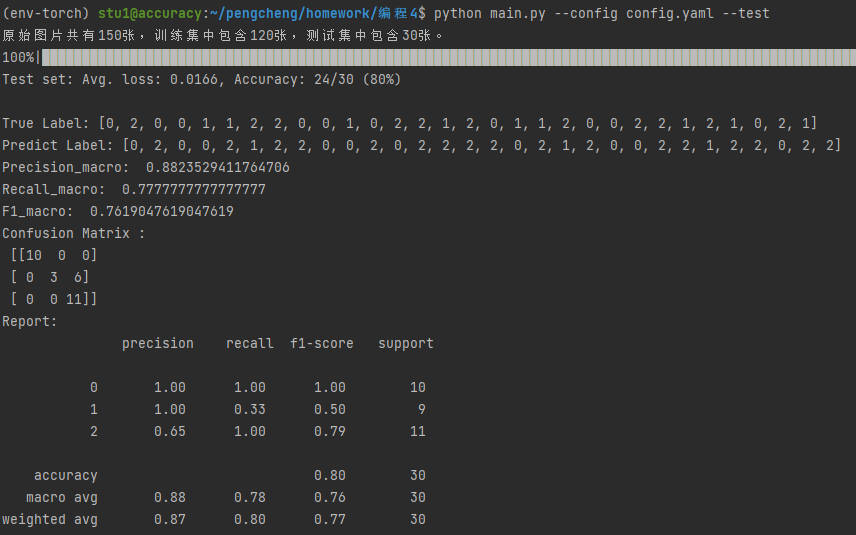
\includegraphics[width=0.9\textwidth]{softmax_result}
  \caption{Softmax结果} 
  \label{Fig.1}
\end{figure}

\begin{figure}[H]
  \centering
  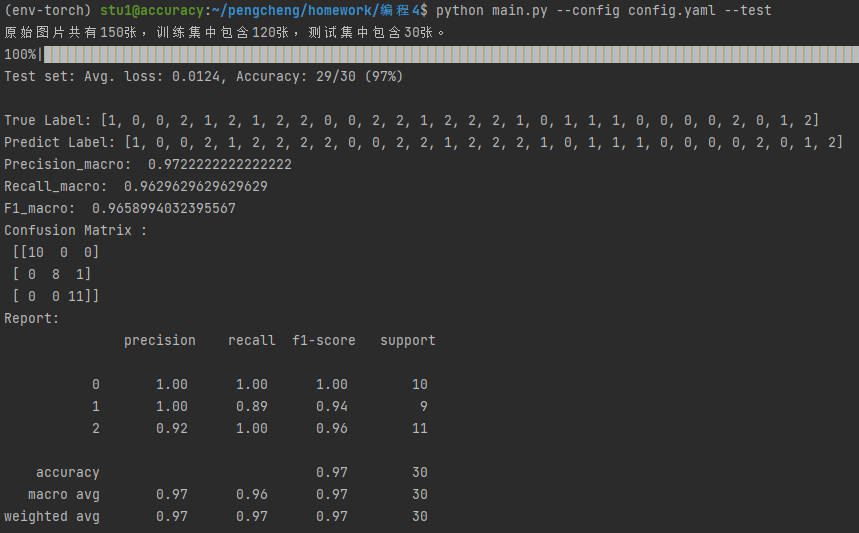
\includegraphics[width=0.9\textwidth]{test_result}
  \caption{MLP结果} 
  \label{Fig.2}
\end{figure}

在数据划分方面,我们划分了20\%的数据用于测试,其余80\%用于训练和验证。

模型在测试集上的测试结果如上述两张图所示,其中Fig \ref{Fig.1}为Softmax模型的结果,Fig \ref{Fig.2}为MLP模型的结果。
其中Softmax模型经过106个epoch后不再提升进入早停,MLP模型经过163个epoch后不再提升进入早停,epoch总数设置为500。

其中Softmax模型经过106个epoch早停后,在测试集上的表现:Accuracy=80\%; Precision=0.88; Recall=0.78; F1=0.76。

MLP模型经过163个epoch早停后,在测试集上的表现:Accuracy=97\%; Precision=0.97; Recall=0.96; F1=0.96。

可以看到MLP模型的表现明显优于Softmax模型,这是因为MLP模型中使用了多个线性层和非线性激活函数,可以刻画更丰富的线性和非线性关系。

\section{总结}

在本次编程作业中,我完成了使用花卉的原始多元特征,在完整数据集上求解三分类问题。通过对比简单softmax模型和MLP模型,增进了对激活函数刻画的非线性关系的理解,同时能够更加熟练地使用pytorch完成实验。

感谢老师和助教的悉心指导!

\nocite{*}
\printbibliography[heading=bibintoc, title=\ebibname]

\appendix
%\appendixpage
\addappheadtotoc

\end{document}
